% \chapter{Challenges and considerations in Federated learning
% }
% \label{Bookchapter}

% \begin{abstract}
% \dropcap{F}ederated learning is a machine learning method that allows decentralized training of deep neural networks among multiple clients while preserving the privacy of each client's data. Federated learning is instrumental in medical imaging due to the privacy considerations of medical data. Setting up federated networks in hospitals comes with its unique challenges, primarily because medical imaging data and federated learning algorithms each have their own set of distinct characteristics. This article introduces federated learning algorithms in medical imaging and discusses technical challenges and considerations of real-world implementation of them.




% \end{abstract}

% \blfootnote{This chapter is partly based on \faFileTextO~\emph{M. Beller. Toward an
%     Empirical Theory of Feedback-Driven Development, ICSE'18 (Student Res
%     earch Competition)}~\cite{BellerSRC2018}.
% }


% \newpage

% \dropcap{T}his is a introductory page.



% keywords can be removed
% \keywords{Federated learning \and Privacy-preserving machine learning \and  Medical imaging}


\section{Introducing FL methods}

With the rapid developments in machine learning in healthcare and computer-aided diagnosis, access to medical data has become a matter of interest. Clinicians, computer scientist and medical technologists require access to more data to enable machine learning based projects. However, there is always a challenging task to balance between building more powerful machines to be used in healthcare industry, and the limitations of accessing large amount of data under the privacy considerations. Generally, sharing data requires hospitals to deal with GDPR restrictions and have an approval from the institutional review board .An institutional review board or ethical committee determines to which degree a hospital can share information with other hospitals and ensures that the GDPR restrictions are complied to. As a result , datacenters in hospitals do not usually have large and diverse datasets required to train deep neural networks. 

Federated learning (FL) \cite{mcmahan2017communication} 
is a machine learning concept proposed by McMahan et al. to tackle this problem. In this concept, a neural network is trained with datasets from multiple hospitals, and the whole training process is managed through a central server. At each round, hospitals train a neural network on their local data, and share the updated models with the central server. The server gathers all the updated models and aggregates them into an updated global model. In the next round, the updated global model is sent back to the hospitals. This way of training enables the researchers to utilize the data from multiple clients, while ensuring that the sensitive data is kept locally. 


There exist several FL algorithms.McMahan et al. \cite{mcmahan2017communication} proposed federated averaging method (FedAvG) to minimize parameter change among hospitals. The algorithm is straightforward: a subset of the clients is selected each round. Training is distributed among multiple clients. Each client will compute an updated model on their own local dataset. All model instances on the clients should start with the same random initialization to achieve convergence. Clients communicate with the central server once their local training has been finished. Finally, the central server gathers the updates of the respective clients. An immediate effect of local training can be seen at this stage. The updated global model can be tested against a test dataset, and comparing its performance with the previous round can give insight into how much improvement was achieved during the last round of training. An illustration of this step is shown in Fig. \ref{fig:train2} Blockchain-based technologies can also be used in the aggregation stage. In a blockchain network, local clients (miners) replace the central server and distribute the aggregation process among themselves. In this case, the whole process will be decentralized. Blockchain networks can be valuable since they prevent failure if the central server or clients fail.\cite{wang2021blockchain} \newpage 
\begin{figure}[h!]
 \centering
  
\includegraphics[scale=0.22]{Training step 2.jpg}
  \caption{Cloud server gathers the locally updated model from clients }
  \label{fig:train2}
\end{figure}


Another approach is averaging the outputs of the local models trained on the clients individually (ensemble single client models).A general definition for ensemble learning is different machine learning algorithms doing the same task are combined into one algorithm. Each algorithm extracts information or features from the input data, and the resulting information will be fused using various mechanisms, such as averaging, and voting. Generally, ensembles consistently outperform each of their consituting algorithms alone. In the federated setting of ensemble learning,  neither the models nor the data will be shared among clients in the training cycle. All the clients will be assigned a similar model with random initial values. Each client will train its model. Their outputs for the same task will be averaged in the deployment phase, resulting in an accumulated knowledge from multiple models.
\begin{figure}[h!]
 \centering
  
\includegraphics[scale=0.32]{Ensemble methods.jpg}
  \caption{Cloud server gathers the locally updated model from clients }
  \label{fig:train2}
\end{figure}


\begin{figure}[h!]
 \centering
  
\includegraphics[scale=0.27]{federated averaging.jpg}
  \caption{Cloud server gathers the locally updated model from clients }
  \label{fig:train2}
\end{figure}


\begin{figure}[h!]
 \centering

\includegraphics[scale=0.3]{SWT.jpg}  \caption{Cloud server gathers the locally updated model from clients }
  \label{fig:train2}
\end{figure}


\begin{figure}[h!]
 \centering

\includegraphics[scale=0.3]{CWT algorithm.jpg}
\caption{Cloud server gathers the locally updated model from clients }
  \label{fig:train2}
\end{figure}


% \begin{figure*}
%      \centering
%      \begin{subcaption}[b]{0.23\textwidth}
%          \centering
%          
\includegraphics[scale=0.32]{Ensemble methods.jpg}
%          \caption{}
%          \label{fig:y equals x}
%      \end{subcaption}
%      \hfill
%      \begin{subfigure}[b]{0.23\textwidth}
%          \centering
%          
\includegraphics[scale=0.27]{federated averaging.jpg}
%          \caption{}
%          \label{fig:three sin x}
%      \end{subfigure}
%      \\ [10pt]
%      \centering
%     %  \hfill
%      \begin{subfigure}[b]{0.21\textwidth}
%          \centering
%          \raisebox{\dimexpr\ht\imagebox-\height}{ \includegraphics[scale=0.3]{SWT algorithm.jpg}}
        
%          \caption{}
%          \label{fig:five over x}
%      \end{subfigure}
%     %  \hspace{0.2\textwidth}
%      \hfill
%      \begin{subfigure}[b]{0.21\textwidth}
%          \centering
%         %  \hfill
%          
\includegraphics[scale=0.3]{CWT algorithm.jpg}
%          \caption{}
%          \label{fig:five over x}
%      \end{subfigure}
%         \centering
%         \captionsetup{justification=centering}
%         \caption{Schema of different decentralized learning methods, (a) Ensemble methods, clients train local models on their own dataset,model outputs of different clients are averaged. (b) FedAvg, an initial model is sent to the clients, each train the model on their own data and the resulting local models are averaged in a central server. (c) SWT, an initial model is sequentially passed through clients and visit each clients once. Final model is the model trained on the latest client. (d) CWT, similar to SWT, however, model is passed through institutions multiple times.}
%         \label{fig:three graphs}
% \end{figure*}




A third algorithm is single weight transfer (SWT). In this algorithm, a deep learning model is trained at a single client up to a particular time and then transferred to the next client. There are numerous options to decide when to finish a local training and pass its model to the next client.  Standard criteria are the number of epochs per client and validation loss or accuracy depending on the problem. For example,  Chang et al. \cite{chang2018distributed} chose to reach the plateau of validation loss as a sign of moving to the next client.  Cyclic weight transfer (CWT) is another algorithm in which a model is trained at each client for a predetermined number of epochs, then transferred to the next client. In this algorithm, the model visits each client than once. 

The functionality of models and tasks in an FL scenario differs depending on the FL algorithm. Algorithms that transfer models are more versatile and adaptable than other algorithms. Deep learning models' performance in a federated environment can also vary from model to model. Models' adaptability can determine the overall performance of an FL network. For example, research has shown that some deep neural network components (such as batch normalization layers) cause performance issues and are harder to adjust in a federated setup. On the other hand, components like convolutional layers could be easily averaged, averaging their results in a proper global model.  As a result, deep learning models that have more suitable components are a better choice for FL. Reseach is going on to develop specific models that perform better in a federated environment\cite{li2021fedbn}.



\subsection{Comparison of the federated learning algorithms}
We may categorize the algorithms based on what is exchanged between the server and the client to compare federated algorithms. Techniques such as FedAVG, SWT, and CWT, transfer the model between the server and the clients. Approaches like split learning \cite{poirot2019split}  transfer middle layer outputs of a neural network. The middle layer outputs can be regarded as a distorted form of the input data. In other words, as the neural network processes the input data, it undergoes numerous modifications that distort the input. Methods such as ensemble methods share their models' final output and broadcast it to a central server. 

The amount of data transferred is relatively tiny in methods in which the model is moved to the central server and is independent of the amount of training data at each site. It is solely determined by the size of the deep learning model. The majority of popular deep learning algorithms are tens of megabytes in size. However, an FL algorithm that transfers a model does not necessarily have a low overall communication overhead. The overall amount of exchanged data also depends on the number of communication rounds between clients and servers. The hyperparameters can determine the number of communication rounds, and communication overhead could be high if there is too much exchange between clients.



% \begin{table*}[h!]
% \centering
% \setlength{\tabcolsep}{8pt}
% \renewcommand\arraystretch{1.4}
% \caption{Result of Average Error Transfer Rate (AETR) for FGSM and PGD methods, with and without CRN initalization }
% % \begin{tabular}{cccccccccccc}
% \begin{tabular}{| *{7}{c|} }\hline

% \setlength\tabcolsep{0pt}
% \begin{table}[h!]
% 	\caption{Comparison of FL methods}
% 	\centering
% 	\setlength{\tabcolsep}{0pt}
%     \renewcommand\arraystretch{1}
%   	\begin{tabular}{|p{0.07} | p{0.05}|p{0.06} |p{0.05}|p{0.10} |p{0.05}|p{0.13} |} \newline
% 		 Methods & Summary & Transferred data & Communication load & Advantages &	Disadvantages &	Usecases \newline
% 		FedAvg$^{*}$ & In each round, every client trains the global model on local data. Then models are averaged &Model &	low	&Easily converged&Weak robustness  with imbalanced clients distribution&COVID-19 CT scans \cite{dou2021federated}
% 		Lung nodule detection  \cite{baheti2020federated} 
%  \newline \hline
%  SWT$^{**}$ &
% 		Model is passed through clients sequentially,visits each client once	&Model&	Very low&	Low communication load&	Highly biased towards the latest institution &	Diabetic retinotherapy  \cite{chang2018distributed}, Mammography  \cite{chang2018distributed}

%       \newline \hline
% 	CWT $\dagger$ &	Model is passed through clients sequentially; the sequence is repeated multiple times&Model&low&High performance&	Needs many rounds to converge&Breast cancer data\cite{beaulieu2018privacy} EHR \cite{beaulieu2018privacy}

%   \newline \hline
% 		Ensemble methods&All the computations are done locally the outputs are averaged&Output&High&Easy to deploy&	High possibility of data leakage, High communication load&Patient health records \cite{li2016distributed} 

%  \newline \hline
% 		CDS$^{\ddagger}$&Move data from clients into a central datacenter&Data&-&High performance&No privacy&MR image reconstruction \cite{Quan2018compressed} , dermoscopy image synthesis \cite{DBLP:journals/corr/abs-1804-03700}
%   \\ \hline
%   \multicolumn{4}{l}{*Federated averaging **Single weight transfer    ${\dagger}$Cyclic weight transfer   $\ddagger$ Centralized data sharing } \\
% 	\end{tabular}
% 	\label{tab:table}
% \end{table}
%     % \begin{tabular}{ll}
%     % \end{tabular}

\begin{table*}[h!]
\centering
\setlength{\tabcolsep}{8pt}
\renewcommand\arraystretch{1.4}






\label{table_core} 
\end{table*}

\begin{figure}[t!]
 \centering
 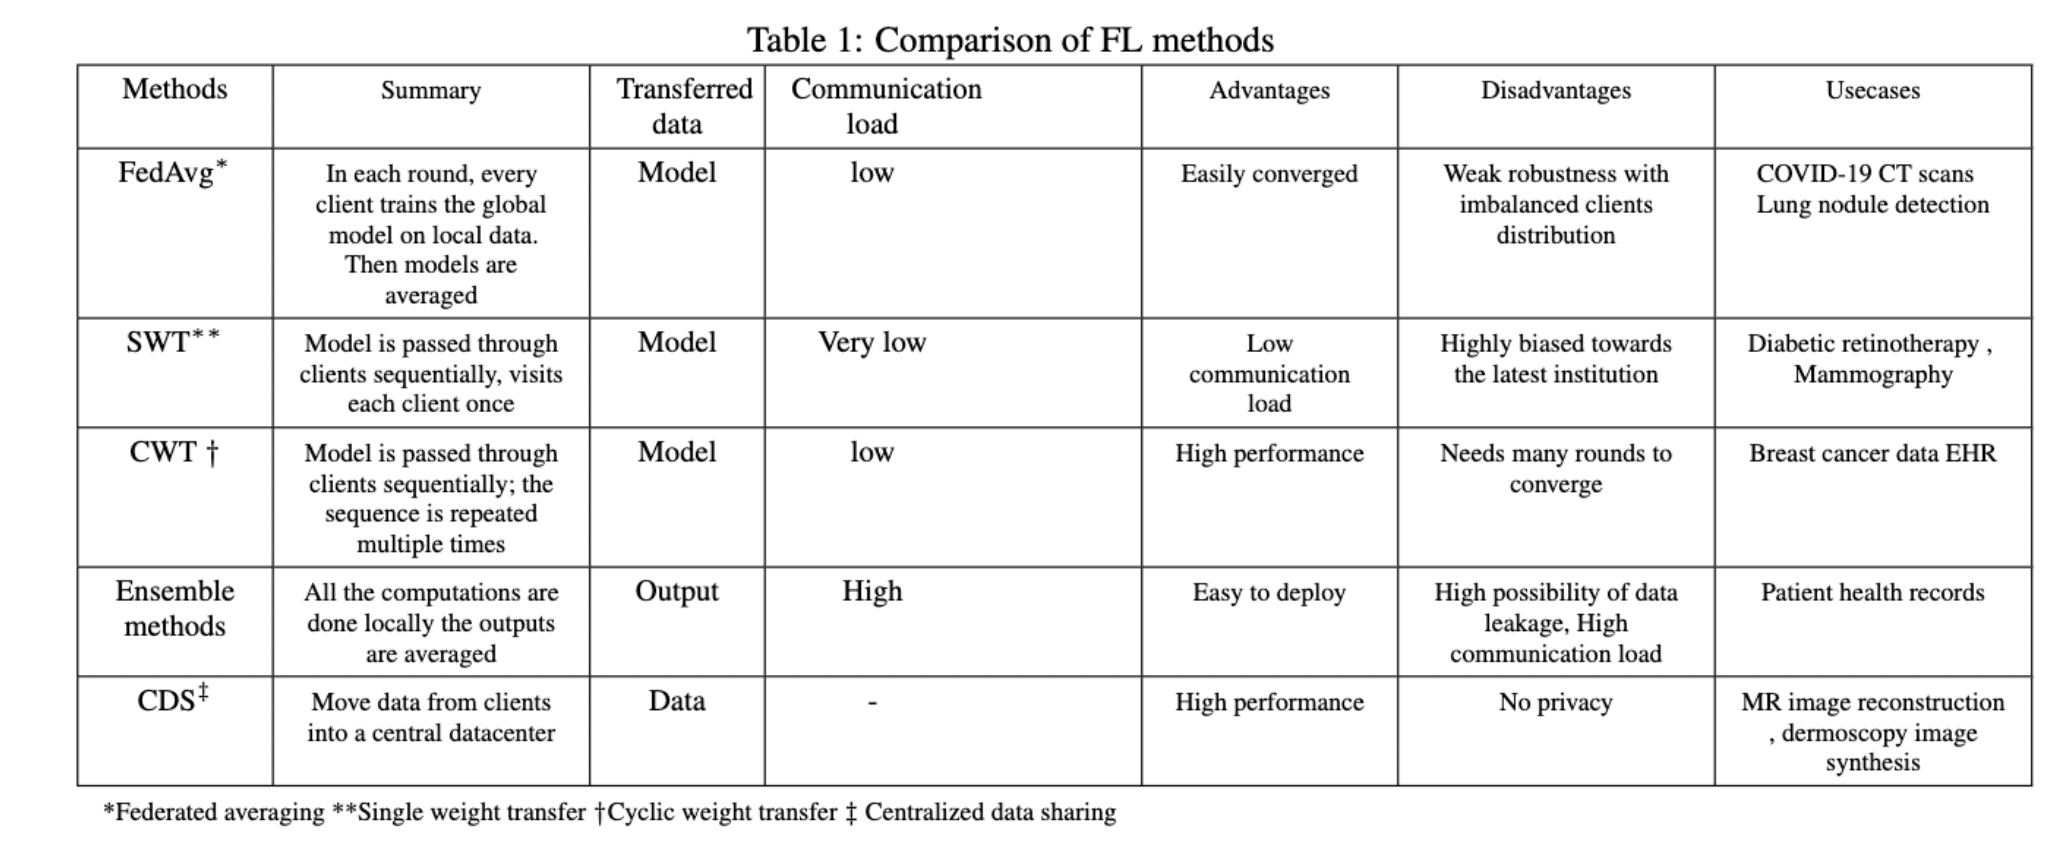
\includegraphics[scale=0.55,angle=90,origin=c]{Chapter3/Screenshot 2022-04-04 at 18.59.31.png}
%  \caption{A schema of adversarial attacks to cancer detection systems}
 \label{fig:pgd-atta-comparison}
\end{figure}

% \begin{table*}[h!]
% \centering
% \setlength{\tabcolsep}{8pt}
% \renewcommand\arraystretch{1.4}
% \caption{Result of Average Error Transfer Rate (AETR) for FGSM and PGD methods, with and without CRN initalization }
% % \begin{tabular}{cccccccccccc}
% \begin{tabular}{| *{7}{c|} }\hline
% % Dataset  & Attack type & \multicolumn{2}{c|}{ $\epsilon=0.01$} & \multicolumn{2}{c|}{ $\epsilon=0.03$}           &    \multicolumn{2}{c|}{ $\epsilon=0.05$}    & \multicolumn{2}{c|}{ $\epsilon=0.07$}                                                              \\ \hline
%  Dataset&\multicolumn{3}{c|}{ FGSM}     &              \multicolumn{3}{c|}{ PGD}                                                                           \\  

%  \cline{2-7}
% &Baseline&CRN5 &CRN10&Baeline&CRN5&CRN10\\\hline

% Meningioma&84.80\%&\textbf{86.31}\%&{84.02}\%&83.73\%  &\textbf{84.25}\%  &84.16\%\\\hline
% Glioma&82.32\% &87.06&\textbf{89.98}&74.89\%&\textbf{83.64}\% &82.32\%\\\hline

% Pathology&\textbf{90.67\%}&{84.81}\%&{85.98}\%&79.86\% &86.79\%&\textbf{86.93\%}\\\hline



% \end{tabular}
% \label{table_core} 
% \end{table*}

% \footnotesize{$^a$ The smallest spatial unit is county, $^b$ more details in appendix A}\\


% (Add the abbreviations with table legend at the bottom of the table)
On the other hand, in algorithms that transfer some type of actual data, whether distorted input data  (e.g., split learning \cite{poirot2019split}) or output data (e.g., ensemble models), the size of sent data can vary greatly depending on the data size. However, because medical imaging data is enormous, the amount of communicated information is usually more significant than with methods that transfer the model. CDS also falls into this category, as it requires actual data transfer to a central server. These two groups differ significantly in terms of communication burden as well as privacy level. Because input/output data is not sent in any format, methods which transfer models are more secure since retrieving patient data from deep learning models is difficult.

In Ensemble models, the ensembling process is done locally, and outputs of the models are sent to the global server instead of model parameters. As a result, heavy server-side computations are avoided and a federated network can be set up easily. Since ensemble models are proven to perform well in various areas of medical imaging, using ensembles can help improve the accuracy, generalizability, and stability of a federated network. However, ensemble methods impose some challenges. First, the risk of data leakage is serious in this setting. Some sort of output data like segmentation masks is very likely to reveal patients' identities. Second, contrary to model size, outputs can vary quite a lot in their size. Outputs in image format require too much communication load. 
In addition, ensemble models are design dependant. Models that do not necessarily share the same objective function can be combined into one ensemble. This leads to one complex multi-objective model having disparate optimization goals. This is not necessarily harmful, but there is a lack of research on the theoretical analysis of ensembles, and the result of an ensemble remains almost always unclear, making ensemble methods unreliable.

Besides, there is always a compromise between training time, model complexity, performance and generelizability. Altough these measures have been thoroughly investigated in single machine learning models, the literature on their relationship in a complex ensemble is still not explored much.



Another aspect of comparing FL models is that FL algorithms, in which a model is transferred, can consistently be averaged by the central server, regardless of the task they are performing. Deep neural networks performing classification, segmentation, regression, or other tasks could be averaged as long as there is a proper deep learning model for that.  All of the mentioned tasks have been demonstrated and proved to work in a federated manner. However, averaging the output from many sources is not always feasible for other federated earning algorithms. For example, if the task is multi-class classification, an ensemble approach cannot simply average the class output of distinct clients. The Ensemble approach is thus limited in the jobs it can tackle.


Several research papers have been published that compare FL implementations. Nilsson et al. \cite{nilsson2018performance} compared various FL methods in practice. They demonstrated that FedAvg is the best FL algorithm. Despite having slightly lower performance than CDS, it is practically comparable in their comparative performance analysis to a non-federated architecture.
There are numerous variants of the FedAvg algorithm and other FL approaches. However, the original FedAvg method remains one of the top methods in comparison studies. Chang et al.\cite{chang2018distributed}investigated several FL algorithms in the radiology area. According to this study, FedAvg does not impose any bias compared to other algorithms because it considers all clients equally and does not arrange them in any particular order. As shown in Figure \ref{fig:three graphs}algorithms such as SWT and CWT, clients are placed in a sequence and trained one after the other. As a result of catastrophic forgetting, the model is more representative of the most recent clients it observed and less of the earlier clients\cite{sheller2020federated}. As a result, there is a bias favoring the most recent institution in models with sequential training. Although CWT can mitigate this effect by running the model through institutions multiple times in a cyclic fashion, bias remains. Table \ref{tab:table} shows the essential characteristics of FL algorithms. There is also a sample of use cases of these algorithms in the medical domain.




Pan et al., \cite{pan2019improving},investigated the impact of the model ensemble for automatic bone age estimation based on imaging data. The results showed that combining heterogenous, uncorrelated models leads to more robust ensembles. Conversely, naively combining top models does not necessarily ensure top-notch performance.
They were able to demonstrate how data FL can aid in identifying comparable patients while protecting their privacy. 
% Another effort was made to explore the structural relationship of the brain without revealing any data. The authors used Principal component analysis (PCA) to uncover anatomical relationships between diverse datasets in a federated setup\cite{grammenos2019federated}. Federated PCA could extract features from MRI pictures from several medical institutes. Their technique was validated using several databases, including ADNI, PPMI, MIRIAD, and UK Biobank\cite{silva2019federated}.

% Balanchandar et al. \cite{balachandar2020accounting} using FL to address the issue of data variability across institutions. They used chest-Xray dataset to classify chest scans. Also, they classified retinotherapy data with their proposed method.




\section{Challenges and considerations}
\label{sec:others}

FL still has a long way to go in radiology. There are numerous challenges both in the theoretical formulation and practical implementation. FL algorithms could be divided into fully decentralized/peer-to-peer methods requiring a trusted central server. Each category comes up with its challenges. Generally speaking, methods with a central server offer more flexibility and better performance, while decentralized methods are more reliable and secure.

However, there is still some risk associated with the FL infrastructure \cite{yin2021see}. An adversary could reconstruct private data from the local model updates\cite{wang2019beyond}. Hospitals can do additional security measures to prevent adversaries from accessing the exchanged data between the server and clients.



\subsection{Data heterogeneity }


The FedAvg algorithm authors claim that their proposed method can handle heterogeneous data. However, the decentralized structure of the data makes data processing challenging to verify the completeness and quality of their findings. Further investigations revealed that this claim is not always valid\cite{li2020federated}. In almost all cases, heterogenous data deteriorates the accuracy of the FL model. The degree of divergence depends on how heterogenous the data is. Local models are trained on data with different patient profiles, resulting in a global model that could not represent all of the profiles. In some cases, heterogenous data prevents model convergence.    


Data homogeneity significantly impacts the version of the federated model to be chosen to train the model. The difference between CDS and FL might vary from similar to CDS better depending on the data. One rule of thumb would be that if data has very different distribution in different data centers, simply averaging each client's data in every round might affect the performance negatively.



Zhao et al.\cite{zhao2018federated}examined the effect of bias that distributing data can have on final performance of FL algorithms. According to their study, difference in data distribution can have negative effect on the model accuracy up to 55\%. Another difficulty is that data heterogeneity might lead to a situation where a best global model might be a poor model for some clients, or a best global model might work quite well on some clients and perform poorly on other clients. Consequently, all participants should agree on the concept of optimum model training in advance of the training. Further technical studies should be carried out to find the optimum technique for updating the central model with heterogeneous data. FedAvg is the standard method for accumulating the data from clients. Still, other distributed optimization methods that can tackle distribution differences are a subject of research.



\subsection{Bias}
Bias is a prevalent issue in distributed networks. Bias is a state that a neural network is inclined towards the distribution of a client more than other clients. It results in the model performing well on that client by compromising the performance on the other clients. The cause of bias could be the difference in the size or the distribution of clients' data. Also, the FL algorithm itself could be a source of bias.


Sheller et al.\cite{sheller2020federated}showed that CWT is a less biased algorithm than SWT. The degree of bias could vary, depending on which client was trained last.They favored FedAvg over SWT and CWT. FedAvg did the FL more fairly.  There is always a bias toward the latest clients they were trained on for algorithms like SWT and CWT. In FedAVG, however, the results of local training are aggregated every round, avoiding bias. In SWT, the global model changes after visiting each client, and succeeding clients mitigate the model's bias towards the preceding institutions. However, there is no mitigation for the latest institution the model is trained on.





The global aggregation method, i.e., server algorithm, should be designed to minimize bias . It also should be robust to local variations, as well as perturbations added by security measures. Reducing bias and designing models that capture diversity is possible by calculating the level of bias arising from each client. Then modifying the  algorithm to address the difference in the distributions. 


However, if the distribution difference is taken into account properly, bias might still emerge later in training. Some features, as well as general data distribution might vary over time.  For example, the number of patients with a particular disease in a particular hospital might change for several reasons. This can cause a domain shift: a change in a client's data distribution. There could be more work on data domain shifts and somehow explicitly address the alterations in gender, patient profile, age, and disease among different institutes or one institute. Models could also be further developed to consider economic or racial status into model training and modify a model to handle diversity in images\cite{li2020multi}. 


\subsection{Lack of standard data}
Standardizing data prevents irrelevant information from being considered meaningful in neural networks. It removes the variability between institutions.  Electronic data management is the norm in medical imaging: and medical communications (DICOM) is the globally recognized image data format and the near-global care standard for electronic file storage. However, not all the available data in the medical imaging sector is standardized. Many institutions still lack the infrastructure to handle their imaging data according to current management standards. 
One factor is the lack of a universal method to organize and manage patient records. Data management is expensive\cite{wang2003cost}. Not all hospitals have advanced data management facilities. This issue leads to the preselection of hospitals participating in research, which is a source of bias.  



Medical data are very diverse because of the diversity of modalities, dimensionalities, and features and because of variables such as variances in the acquisition, medical equipment brand, or local demographics within a specific protocol. There is still no uniform data standardization method. As a result, healthcare federated networks are likely to have clients with disparate data quality and distribution. Methods like FedAvg are generally likely to fail under these circumstances.  One way to avoid bias is to harmonize data and make each client data type similar, following a similar preprocessing. This also might require sharing metadata among institutions to find a general method of harmonization in data that suits all the institutions. But this could be tricky given the restrictions of individual institutions. Hence, one way of further development for FL systems is that the clinicians and computer scientists collaborate to standardize handling data among multiple institutions concerning the privacy restrictions and considerations.



\subsection{Privacy and Security}
Data breach is a major concern and medical data and must be safeguarded in compliance with accepted confidentiality procedures. FL has proven to be effective in protecting patients' privacy and anonymity by keeping data locally. However, there are some privacy-related challenges associated with FL. Despite many attempts to de-identify personal data from DICOM images, patient information could still be re-identified\cite{Peter2015Free} \cite{monteiro2015machine}. Recent studies have successfully rebuilt a patient's face from their MRI data. Furthermore, adversaries could steal the data or access the algorithm for non-encrypted networks. 


Furthermore, deep learning models still have some sensitive information in the weights they carry. On a decentralized network, it is feasible to reconstitute portions of patients' information only having the local model from one client\cite{carlini2019secret} \cite{zhang2020secret}
\cite{hitaj2017deep}. Adversaries can decrypt deep learning models and reveal patients' information with a very high accuracy\cite{fredrikson2015model}. Malicious parties can distort the deep learning models. False outputs produced by such models can have severe consequences if used in practice. As a result, it should be ensured that models are secure and that adversaries cannot breach models to be employed in the real-world setting\cite{tomsett2019model}.



There are specific measures to improve privacy. Particular countermeasures, such as model encryptions, Differential privacy (DP), \cite{abadi2016deep} adversarial defense against malicious clients,\cite{hitaj2017deep} and increased communication security, can be done. DP refers to the practice of keeping a dataset's global statistical distribution while minimizing individually identifiable information. DP can be done by adding perturbation to each sample.Adding noise to a dataset to reduce the chance of private data being revealed is based on the argument that one can preserve general data distribution while individual samples are changed by randomly altering a dataset. Adding systematic noise helps machine models to learn the whole distribution of training data while keeping each sample anonymous.


However, such countermeasures complicate the training algorithms and can affect training performance. Sometimes much longer training times are required, or accuracy will be dramatically decreased. This can impose an additional cost on the whole network. Hence, it is quintessential to consider whether deploying a countermeasure is necessary. The cost-efficiency of implementing them depends mainly on the level of trust among involved parties and the project scale. If clients do not trust each other, then DP is a necessity. This is because federated clients have regular communication, and critical information can be exchanged in the interactions. So each client's data should be safeguarded from other clients. This shows how important it is to clarify the level of trust among clients. This argument holds true in fully decentralized algorithms, where no central node is involved. And also in algorithms including a central server, where the client/server trust is also essential. 
Total image anonymization is still a problem. In the absence of encryption, attackers may acquire private information from local datacenters or intercept the communication pathways and rob the passing data.


\subsection{System architecture}

Medical data in federated networks requires on-premise or cloud-based data storage. Hospitals might need private or cloud-based computing power. As well as software for preprocessing and standardization of data, such as PACS. To allow the local model training hardware (GPU), connections and data centers should be set up in local centers. These bring their challenges, such as high computational power to assure harmony with other clients and high-performance bandwidth and connection between different centers, which is not always feasible in medical centers. Many hospitals still lack computing resources and strong internet connections \cite{li2010securing}. Besides, for the whole network to work correctly, redundant computational facilities and data centers should be devised to prevent data loss. If one computational client fails, the network could continue its training, which imposes an additional challenge. Robustness of the network is also critical ;federated models should be structured so that adding or removing clients and increasing or decreasing the amount of data in a center does not negatively impact patient data or model privacy.

\section{Conclusion}
 

This article introduced the main federated learning algorithms used in radiology and compared their characteristics.  
A Federated setting faces myriad challenges; designing algorithms to address them results in various algorithms with distinct optimization objectives. In general, developments focus on privacy, communication load, data heterogeneity, and model performance as their objective. This paper discusses and compares federated learning algorithms based on these objectives. We start by introducing federated learning and its paramount role in medical imaging research. Then we present the most popular federated learning algorithms and compare them.
We discuss several challenges and considerations in the next section. These challenges are current lines of research and require extra attention in implementing federated learning networks.

\printbibliography

% \bibliographystyle{unsrtnat}
% \bibliography{dissertation} 
% I hope this helps you get started!
% Moritz
